\documentclass[a4paper,10pt]{article}
\usepackage{fullpage, comment, bookman, lastpage, fancyhdr, listings, color, graphicx, float}
\usepackage[hidelinks]{hyperref}
\usepackage[ddmmyy]{datetime}
\pagestyle{fancy} \fancyhf{} \renewcommand{\headrulewidth}{0pt} \cfoot{\thepage\ of \pageref{LastPage}}
\setlength\parindent{0pt}

\specialcomment{answer}{\begingroup \color{blue}}{\endgroup}
\newcommand{\mystar}{\hspace{-2em}{$\star$}\hspace{1.5em}}
\includecomment{comment}

\lstdefinelanguage{JavaScript}{
	morecomment=[l]{//},
	morecomment=[s]{/*}{*/},
	morestring=[b]',
	morestring=[b]",
	ndkeywords={class, export, boolean, throw, implements, import, this},
	sensitive=true
}

\lstset{
	language=JavaScript,
	extendedchars=true,
	basicstyle=\footnotesize\ttfamily,
	showstringspaces=false,
	showspaces=false,
	numbers=left,
	numberstyle=\footnotesize,
	numbersep=9pt,
	tabsize=2,
	breaklines=true,
	showtabs=false,
	captionpos=b
}

\lstdefinelanguage{docker}{
	keywords={FROM, RUN, COPY, ADD, ENTRYPOINT, CMD,  ENV, ARG, WORKDIR, EXPOSE, LABEL, USER, VOLUME, STOPSIGNAL, ONBUILD, MAINTAINER},
	keywordstyle=\color{blue}\bfseries,
	identifierstyle=\color{black},
	sensitive=false,
	comment=[l]{\#},
	commentstyle=\color{purple}\ttfamily,
	stringstyle=\color{red}\ttfamily,
	morestring=[b]',
	morestring=[b]"
}

\newcommand\YAMLcolonstyle{\color{red}\mdseries}
\newcommand\YAMLkeystyle{\color{black}\bfseries}
\newcommand\YAMLvaluestyle{\color{blue}\mdseries}
\makeatletter
% here is a macro expanding to the name of the language
% (handy if you decide to change it further down the road)
\newcommand\language@yaml{yaml}

\expandafter\expandafter\expandafter\lstdefinelanguage
\expandafter{\language@yaml}
{
	keywords={true,false,null,y,n},
	keywordstyle=\color{darkgray}\bfseries,
	basicstyle=\YAMLkeystyle,                                 % assuming a key comes first
	sensitive=false,
	comment=[l]{\#},
	morecomment=[s]{/*}{*/},
	commentstyle=\color{purple}\ttfamily,
	stringstyle=\YAMLvaluestyle\ttfamily,
	moredelim=[l][\color{orange}]{\&},
	moredelim=[l][\color{magenta}]{*},
	moredelim=**[il][\YAMLcolonstyle{:}\YAMLvaluestyle]{:},   % switch to value style at :
	morestring=[b]',
	morestring=[b]",
	literate =    {---}{{\ProcessThreeDashes}}3
	{>}{{\textcolor{red}\textgreater}}1     
	{|}{{\textcolor{red}\textbar}}1 
	{\ -\ }{{\mdseries\ -\ }}3,
}

% switch to key style at EOL
\lst@AddToHook{EveryLine}{\ifx\lst@language\language@yaml\YAMLkeystyle\fi}
\makeatother
\newcommand\ProcessThreeDashes{\llap{\color{cyan}\mdseries-{-}-}}

\begin{document}
	
\textbf{Distributed and Pervasive Systems. Exercises} \hfill \today, \currenttime\\
Session 01-02: Cloud computing\\
Christian Marius Lillelund, cl@ece.au.dk\\
\hrule

\section{Exercise 1 - Setting up minikube}
		
We'll start by setting up a single-node Kubernetes cluster with Minikube. Setting up a full-fledged, multi-node Kubernetes cluster isn't a trivial task and requires a good amount of expertise in Linux and networking. Therefore we'll stick to minikube here, since it is the simplest and quickest path to a fully functioning Kubernetes cluster. In a real enterprise application, Kubernetes is usually set up in a cloud environment (like Google Cloud and Amazon AWS) instead of a local workstation, but for exercise purposes it works just fine. \\

Step 1: Docker is prerequisite to minikube, so we need that first. Docker can be downloaded here for various OS and architectures:

\url{https://hub.docker.com/search?q=&type=edition&offering=community} \\

Step 2: We can now install minikube. Instructions are available in the Kubernetes documentation. Choose your OS and follow along. For most Windows users, the Windows installer will do fine:

\url{https://kubernetes.io/docs/tasks/tools/install-minikube/} \\

The Kubernetes docs will instruct you to download a Hypervisor before installing minikube, but if you're on Windows 10 this is not necessary, as it is already included in Windows 10. This may be the case for macOS/Linux users as well.

Step 3: Assuming the installation went well, then from a terminal with administrator access type:

\begin{lstlisting}[numbers=none, basicstyle=\ttfamily]
$ minikube start
\end{lstlisting}

This should produce output similar to this:

\begin{lstlisting}[numbers=none, basicstyle=\ttfamily]
Starting local Kubernetes cluster...
Running pre-create checks...
Creating machine...
Starting local Kubernetes cluster...
\end{lstlisting}

Step 4: We can now use kubectl to access our new cluster. To verify it is working, you can use the \textit{kubectl cluster-info} command in the following listing:

\begin{lstlisting}[numbers=none, basicstyle=\ttfamily]
$ kubectl cluster-info
Kubernetes master is running at https://192.168.99.100:8443
KubeDNS is running at https://192.168.99.100:8443/api/v1/proxy/...
kubernetes-dashboard is running at https://192.168.99.100:8443/api/v1/...
\end{lstlisting}

This shows everything is set up and running. We'll get to actually deploying software and and containers in the next exercises. As a bonus feature, minikube bundles the Kubernetes Dashboard, which you can launch with the following command to see a ton of information about your new environment:

\begin{lstlisting}[numbers=none, basicstyle=\ttfamily]
$ minikube dashboard
\end{lstlisting}

That's it for exercise 1. You now have a working cluster with minikube.

\pagebreak

\section{Exercise 2 - Building and deploying with Docker}

In this exercise we will explore Docker and use it to build our first real container application. In all essence, Docker toolkit comes in two parts: The \textbf{Docker Engine} and the \textbf{Docker Client}. The Docker Engine allows you to develop, assemble, ship, and run applications, whereas the Docker client enables users to interact with Docker. The Docker client can reside on the same host as the daemon or connect to a daemon on a remote host. A docker client can communicate with more than one daemon. The Docker client provides a command line interface (CLI) that allows you to issue build, run, and stop application commands to a Docker daemon. Its main purpose is to provide the means to direct the pull of images from a registry and to have it run on a Docker host. Common commands issued by a client are: \\

docker build \\
docker pull \\
docker run \\

See more about Docker's architecture here: \url{https://wiki.aquasec.com/display/containers/Docker+Architecture} \\

Step 1: We want to first run a simple Hello World container with Docker and then use the Docker client to make our own container image - which we'll later deploy to Kubernetes and run in a managed environment. The public Docker container registry, Docker Hub, contains ready-to-use container images for many well-known software packages. One of them is the busybox image, which we'll use to run a simple "Hello world" command. Use the \textit{docker run} command and specify the busybox image and what command it should execute, like this (remember to start Docker!):

\begin{lstlisting}[numbers=none, basicstyle=\ttfamily]
$ docker run busybox echo "Hello world"
Unable to find image 'busybox:latest' locally
latest: Pulling from library/busybox
61c5ed1cbdf8: Pull complete
Digest: sha256:4f47c01fa91355af2865ac10...
Status: Downloaded newer image for busybox:latest
Hello world
\end{lstlisting}

This downloads and executes the whole app in a single command. Figure \ref{fig:dockerhelloworld} shows what happens behind the scenes when you execute the command.\\

\begin{figure}
	\centering
	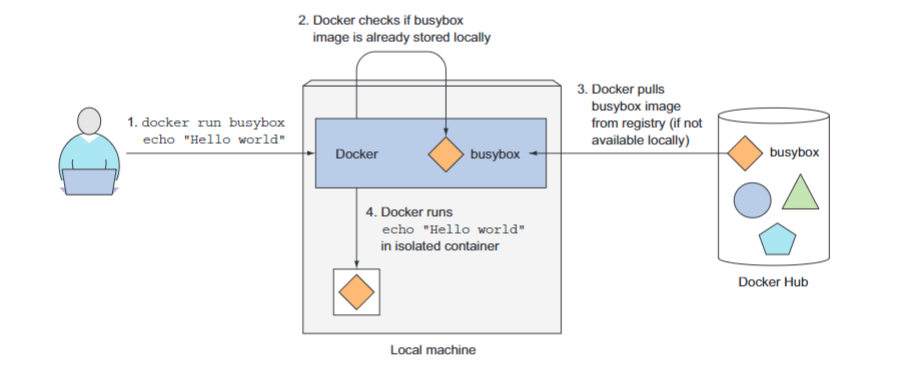
\includegraphics[width=0.8\linewidth]{docker_hello_world}
	\caption{How the busybox image gets downloaded and executed.}
	\label{fig:dockerhelloworld}
\end{figure}

Step 2: Now that we have a working Docker setup, we can make our own application, package it into a container image and run it on Docker. And later deploy it to Kubernetes, of course. We'll build a trivial Node.js web application here. The application will accept HTTP requests and respond with the hostname of the machine its running  in. We'll see, that an app running  inside a container sees its own hostname and not that of the host machine, even though it's running on the host. This will be useful later, when we deploy the app on Kubernetes and scale it out (run multiple instances of the app). The app will consist of a single file called app.js, so create that on your computer and add the content below:

\begin{lstlisting}[language=JavaScript, numbers=none, frame=single]
const http = require('http');
const os = require('os');

console.log("Kubia server starting...");

var handler = function(request, response) { 
	console.log("Received request from " + request.connection.remoteAddress);
	response.writeHead(200);
	response.end("You've hit " + os.hostname() + "\n");
};
var www = http.createServer(handler);
www.listen(8080);
\end{lstlisting}

This code starts up a HTTP server on port 8080. The server responds with an HTTP response status code 200OK and the text "You've hit hostname" to every request. To run the app, normally you would need to download Node.js and trouble yourself with installing dependencies, but not with Docker: We can simply package the app into a container image using Docker and enable it to be run anywhere without having to download or install anything (only Docker). Next we'll make a Dockerfile for the app. \\

Step 3: To package our app into an image, we first need to create a Dockerfile, which will contain a list of instructions  that Docker will perform when building the image. The Dockerfile needs to be in the same directory as the app.js file and should contain the commands shown below:

\begin{lstlisting}[language=Docker, numbers=none, frame=single]
FROM node:7
ADD app.js /app.js
ENTRYPOINT ["node", "app.js"]
\end{lstlisting}

The \textit{FROM} line defines the container image we'll use as a starting point (the base image). Here, we're using a node base image with tag 7. In the second line, we're adding the app.js file from our local directory into the root directory of the image, under the same name (app.js). Finally, in the third line, we're defining what command should be executed when  somebody runs the image. In this case, the command is \textit{node app.js}. \\

Step 4: Now we're ready to build the image. Open a terminal in the directory where the app.js and Dockerfile files are and build the image using Docker:

\begin{lstlisting}[numbers=none, basicstyle=\ttfamily]
$ docker build -t kubia .
\end{lstlisting}

Our image should now be available in our local Docker repository:

\begin{lstlisting}[numbers=none, basicstyle=\ttfamily]
$ docker images
REPOSITORY   TAG      IMAGE ID           CREATED             VIRTUAL SIZE
kubia        latest   d30ecc7419e7       1 minute ago        637.1 MB
\end{lstlisting}

We can now run our image with the following command:

\begin{lstlisting}[numbers=none, basicstyle=\ttfamily]
$ docker run --name kubia-container -p 8080:8080 -d kubia
\end{lstlisting}

This tells Docker to run a new container called kubia-container from the kubia image we just built. The container will be detached from the console (-d flag), which means it will run in the background. Port 8080 on our local machine will be mapped to port 8080 inside the container (-p 8080:8080 option), so we can now access the app at: \url{http://localhost:8080} in a browser or use curl from a terminal:

\begin{lstlisting}[numbers=none, basicstyle=\ttfamily]
$ curl localhost:8080
You've hit 44d76963e8e1
\end{lstlisting}

Our tiny application is now running inside a container, isolated from everything else. It's returning its hostname 44d76963e8e1, which is not the hostname of the host machine, but the ID of the docker container. To list all running containers on Docker, simply run:

\begin{lstlisting}[numbers=none, basicstyle=\ttfamily]
$ docker ps
\end{lstlisting}

A single container is running, the one we've just deployed. For each container, Docker prints out its ID and name, the image used to run the container, and the command that's executing inside the container. To stop our app, we'll use Docker to stop the kubia-container container by:

\begin{lstlisting}[numbers=none, basicstyle=\ttfamily]
$ docker stop kubia-container
\end{lstlisting}

This will stop the main process running in the container, but not remove the actual container from the system. You can still see it with the\textit{ docker ps} command. To truly remove the container, we need to remove it with the \textit{docker rm} command:

\begin{lstlisting}[numbers=none, basicstyle=\ttfamily]
$ docker rm kubia-container
\end{lstlisting}

Step 5: In order to run our image in Kubernetes, we need to push it to Docker Hub, so that Kubernetes can download and execute it. What you need to do first is to go Docker Hub at \url{http://hub.docker.com} and create an account. You'll need a Docker ID to properly tag the containers you push to Docker Hub according to their rules. Docker Hub only allows you to push an image if the image's repository name starts with your Docker Hub ID. Once you know your ID, let's rename the previous image from \textit{kubia} to \textit{dockerid/kubia}, where \textit{dockerid} is your Docker ID:

\begin{lstlisting}[numbers=none, basicstyle=\ttfamily]
$ docker tag kubia <dockerid>/kubia
\end{lstlisting}

Confirm that you have successfully created an additional tag for the kubia image by running (unimportant information is omitted). Note that now \textit{kubia} and \textit{luksa/kubia} points to the same image ID.

\begin{lstlisting}[numbers=none, basicstyle=\ttfamily]
$ docker images
REPOSITORY    	TAG     IMAGE ID         CREATED           SIZE
dockerid/kubia  latest  d30ecc7419e7     5 minutes ago	   660MB
kubia           latest  d30ecc7419e7     5 minutes ago	   660MB
\end{lstlisting}

Let's push the image to Docker Hub by first logging in and then pushing it:

\begin{lstlisting}[numbers=none, basicstyle=\ttfamily]
$ docker login
Authenticating with existing credentials...
Login Succeeded
$ docker push dockerid/kubia
\end{lstlisting}

After the push to Docker Hub is complete, the image will be available to everyone. You can go online and see the image in your own repository at Docker Hub. Your friends can run your images on their computers and you can run their images on your computer. To run the image, execute the following command:

\begin{lstlisting}[numbers=none, basicstyle=\ttfamily]
$ docker run -p 8080:8080 -d <dockerid>/kubia
\end{lstlisting}

That's it for exercise 2. You now know the basics behind Docker, how to build a new image from a Dockerfile and how to deploy it to Docker Hub. You also learned how to execute it locally on Docker. In the next exercise we'll deploy the image to Kubernetes. Remember stop the kubia container before continuing.

\pagebreak

\section{Exercise 3 - Our app in Kubernetes}

In this exercise we'll dig a bit deeper into Kubernetes and try to run pods and deployments on it. We'll also see how we can create, edit and deploy a YAML file that describes a Kubernetes resource, such as a deployment. We'll use the \textit{kubectl} as well to create services that can act as load-balancers for our pods and try scaling our system. Since we've already set up minikube in exercise 1, we're ready to use Kubernetes. \\

Step 1: First we'll create a Kubernetes pod based on the simple Node.js app we made previously and pushed to Docker Kub. Recall that a pod is a group of one or more tightly-coupled containers and a pod is usually operated by a ReplicationController or Deployment. For now, we'll just create a stand-alone pod:

\begin{lstlisting}[numbers=none, basicstyle=\ttfamily]
$ kubectl run kubia --image=<dockerid>/kubia --port=8080 --generator=run-pod/v1
pod/kubia created
\end{lstlisting}

As the previous command's output shows, a pod called \textit{kubia} has been created. We can verify this by executing the \textit{get pods} command, which should tell us that the pod is up and running:

\begin{lstlisting}[numbers=none, basicstyle=\ttfamily]
$ kubectl get pods
NAME	READY   STATUS    RESTARTS   AGE
kubia 1/1     Running   0          1m
\end{lstlisting}

It takes some time to download the image first time, so if your pod says \textit{ContainerCreating}, wait a few moments until the download's complete and rerun the command. It should show a running status. You can use the \textit{kubectl describe pod} command to get more details about the pod, if you like. Now, for us to access the pod, we'll need to create a service, so we'll do that next. \\

Step 2: A pod in Kubernetes get its own IP, but that IP is internal to the cluster and cannot be accessed from outside. In order for us to do so, we need to make a Service object. We'll create a special service of type NodePort, so that we'll expose the service on an internal IP in the cluster. To create the service, run:

\begin{lstlisting}[numbers=none, basicstyle=\ttfamily]
$ kubectl expose pod kubia --type=NodePort --name kubia-http
service/kubia-http exposed
\end{lstlisting}

We have now made a service called kubia-http. We can use the \textit{kubectl get service} command to see it:

\begin{lstlisting}[numbers=none, basicstyle=\ttfamily]
$ kubectl get services
NAME	       TYPE	          CLUSTER-IP	    EXTERNAL-IP	 PORT(S)
kubernetes   ClusterIP      10.96.0.1       <none>       443/TCP
kubia-http   NodePort       10.99.156.171   <none>       8080:32583/TCP
\end{lstlisting}

If we ignore the \textit{kubernetes} service and focus on our kubia-http service, we see that Kubernetes has assigned a cluster IP to it and bound the pod's HTTP port 8080 to 32583 of our host. Now, the cluster IP is internal to Kubernetes, so you won't be able to access that, and since we're running minikube on our own personal computer, there is no such thing as an external IP. In a real cluster, you would use a \textit{LoadBalancer} service here and bind it to an external IP that your clients can access, but minikube does not support that, so we'll just use the \textit{NodePort} version. To access our pod through the service, we need to know the URL, so let's find it (this may be a different IP for you):

\begin{lstlisting}[numbers=none, basicstyle=\ttfamily]
$ minikube service kubia-http --url
http://172.17.248.28:32583
\end{lstlisting}

Use curl or your favorite web browser to access the pod. Alternatively, minikube has a helper function that does all this in one go, if you run \textit{minikube service kubia-http}.

\begin{lstlisting}[numbers=none, basicstyle=\ttfamily]
$ curl http://172.17.248.28:32583
\end{lstlisting}

The app is reporting the name of the pod as its hostname, since each pod behaves like a separate independent machine with its own IP address and hostname. Even though the application is running in the worker node's operating system, to the app it appears as though it's running on a separate machine.

Now, delete the service and pod we just created, since we'll turn our attention to deployments next:

\begin{lstlisting}[numbers=none, basicstyle=\ttfamily]
$ kubectl delete service kubia-http
service "kubia-http" deleted
$ kubectl delete pod kubia
pod "kubia" deleted
\end{lstlisting}

Step 3: Deployments is one of the cornerstones of Kubernetes. They are a newer and higher level concept than ReplicationControllers, which you may have read about, and are intended to replace ReplicationControllers.  They make it easy to deploy pods, roll out changes and do a roll-back if necessary. They can be deployed either declaratively in the terminal or with a YAML configuration file. You can find a good source of information about Deployments and Services in the online docs. They use the YAML approach, which we'll get to in Step 4. For now, we'll just use the terminal. \\

Deployment: \url{htt://kubernetes.io/docs/concepts/workloads/controllers/deployment/} \\
Service: \url{https://kubernetes.io/docs/concepts/services-networking/service/} \\

Let's create a deployment in the terminal:

\begin{lstlisting}[numbers=none, basicstyle=\ttfamily]
$ kubectl create deployment kubia-deployment --image=<dockerid>/kubia
deployment.apps/kubia-deployment created
\end{lstlisting}

We'll verify our deployment using the \textit{kubectl get deployments} command:

\begin{lstlisting}[numbers=none, basicstyle=\ttfamily]
$ kubectl get deployments
NAME               READY   UP-TO-DATE   AVAILABLE   AGE
kubia-deployment   1/1     1            1           41s
\end{lstlisting}

Our deployment is ready and running in one pod. Now let's create a service for it like before:

\begin{lstlisting}[numbers=none, basicstyle=\ttfamily]
$ kubectl expose deployment kubia-deployment --type=NodePort --port=8080 --target-port=8080 --name=kubia-service
service/kubia-deployment exposed
\end{lstlisting}

Use minikube's helper function to get the IP for the service (the IP may differ at your end):

\begin{lstlisting}[numbers=none, basicstyle=\ttfamily]
$ minikube service kubia-deployment --url
http://172.17.248.28:32358
$ curl http://172.17.248.28:32358
\end{lstlisting}

When you access the service, the pod replies with it's hostname and its unique ID as a suffix. Every time you curl, you will access the same pod, since there's only one right now. Let's try using Kubernetes scaling feature to create multiple instances of our application - pods. This way, if one of the pods stops working, the service will simply forward incoming requests to another:

\newpage

\begin{lstlisting}[numbers=none, basicstyle=\ttfamily]
$ kubectl scale deployment kubia-deployment --replicas=5
$ kubectl get pods
NAME                   READY   STATUS              RESTARTS   AGE
kubia-deployment-...   1/1     Running             0          4s
kubia-deployment-...   1/1     Running             0          17m
kubia-deployment-...   0/1     ContainerCreating   0          4s
kubia-deployment-...   0/1     ContainerCreating   0          4s
kubia-deployment-...   0/1     ContainerCreating   0          4s
\end{lstlisting}

The pods should soon come up and when they do, we can access them through our service. Recall that us (the client) do not talk directly with the pods, but with the service. Thus we are unaware of how many pods the system has and what their status are. We simply ask the service to provide us the application and it will forward our request to the first working pod in a round-robin fashion. One thing to note is that requests belonging to the same session gets routed to the same pod every time, so if you want to see other pods responding, you'd have to make a new session. Try starting a different browser and you should start seeing different pods responding to your request. 

\begin{lstlisting}[numbers=none, basicstyle=\ttfamily]
$ curl http://172.17.248.28:32358
\end{lstlisting}

Let's go back to just one pod:

\begin{lstlisting}[numbers=none, basicstyle=\ttfamily]
$ kubectl scale deployment kubia-deployment --replicas=1
$ kubectl get pods
NAME                   READY   STATUS        RESTARTS   AGE
kubia-deployment-...   1/1     Terminating   0          8m15s
kubia-deployment-...   1/1     Running       0          25m
kubia-deployment-...   1/1     Terminating   0          8m15s
kubia-deployment-...   1/1     Terminating   0          8m15s
kubia-deployment-...   1/1     Terminating   0          8m15s
\end{lstlisting}

If you want a more detailed look at the many other details of a pod, use \textit{kubectl describe}. Note that all pods are running on the same minikube node, as we do not have multiple nodes.

\begin{lstlisting}[numbers=none, basicstyle=\ttfamily]
$ kubectl describe pod <pod_name>
Name:         kubia-deployment-6fdb84979b-7krb8
Namespace:    default
Priority:     0
Node:         minikube/172.17.248.28
...
\end{lstlisting}

For the next and final step, we'll create a deployment specification in a YAML file and deploy it. Delete the service and deployment before continuing. \\

Step 4: A Deployment provides declarative updates for Pods. You describe a desired state in a Deployment file or inline, and the DeploymentController changes the actual state to the desired state at a controlled rate. You can define Deployments to create new pods, or to remove existing ones and adopt all their resources with new Deployments. The way to make new Deployments is by creating and applying YAML configuration files, that contain the entire Deployment specification. All you need in order to have a working end-to-end system is a Docker image, a Deployments YAML file and a service. We'll look at an example YAML file for the Kubia deployment now:

\newpage

\begin{lstlisting}[language=yaml, numbers=none, frame=single]
apiVersion: apps/v1
kind: Deployment
metadata:
	name: kubia-deployment
	labels:
		app: kubia
spec:
	replicas: 3
	selector:
		matchLabels:
			app: kubia
	template:
		metadata:
			labels:
				app: kubia
		spec:
			containers:
			- name: kubia
			  image: <dockerid>/kubia
			  ports:
			  - containerPort: 8080
\end{lstlisting}

We'll create the YAML above as a kubia-deployment.yml file and save it on our computer. You can find all YAML's in this repository to save time: \url{https://github.com/thecml/kubernetes-exercises}. \\

When you've created the file, simply deploy it with \textit{kubectl apply}:

\begin{lstlisting}[numbers=none, basicstyle=\ttfamily]
$ kubectl apply -f .\kubia-deployment.yml
\end{lstlisting}

This will create a deployment like before with 3 replicas based on the dockerid/kubia image. Since we want a service as well, we can make the one we used before, but now based on a kubia-service.yml file:

\begin{lstlisting}[language=yaml, numbers=none, frame=single]
apiVersion: v1
kind: Service
metadata:
	name: kubia-service
spec:
	type: NodePort
	selector:
		app: kubia
	ports:
		- protocol: TCP
		  port: 8080
		  targetPort: 8080
\end{lstlisting}

Apply the service file similarly:

\begin{lstlisting}[numbers=none, basicstyle=\ttfamily]
$ kubectl apply -f .\kubia-service.yml
\end{lstlisting}

You now have a deployment and a service made entirely out of YAML files. Using YAML for Kubernetes definitions gives us a number of advantages: We no longer have to add all of our parameters to the command line, we can add the YAML files to source control (Git) and we're able to create much more complex structures using YAML than we can using the command line. Configuration files grow quickly in an enterprise setup, so versioning and usability is important.

\end{document}